\documentclass[9pt,a4paper]{article}

% Packages
\usepackage[utf8]{inputenc}
\usepackage[T1]{fontenc}
\usepackage{amsmath}
\usepackage{amsfonts}
\usepackage{amssymb}
\usepackage{graphicx}
\usepackage{hyperref}
\usepackage{geometry}
\usepackage{multicol}
\usepackage{xcolor}
\usepackage{enumitem}
\usepackage{tikz}
\usetikzlibrary{calc}

% Page setup
\geometry{a4paper,landscape,left=0.2cm,right=0.2cm,top=0.2cm,bottom=0.2cm}
\setlength{\columnsep}{0.1cm}
\pagestyle{empty}

% Typography and spacing
\setlength{\parindent}{0pt}
\setlength{\parskip}{0.3em}
\setlength{\baselineskip}{0.9em}
\setlist{nosep,leftmargin=*,itemsep=0.1em,parsep=0.1em}

% Section formatting - compact, no numbering
\setcounter{secnumdepth}{0}
\makeatletter
\renewcommand{\section}{\@startsection{section}{1}{0pt}{0.5em}{0.3em}{\normalfont\bfseries\large}}
\renewcommand{\subsection}{\@startsection{subsection}{2}{0pt}{0.4em}{0.2em}{\normalfont\bfseries\normalsize}}
\makeatother

% Compact equation spacing
\setlength{\abovedisplayskip}{0.3em}
\setlength{\belowdisplayskip}{0.3em}
\setlength{\abovedisplayshortskip}{0.2em}
\setlength{\belowdisplayshortskip}{0.2em}

% Custom commands for cheatsheet formatting
\newcommand{\definition}[2]{\textbf{#1:} #2\par}
\newcommand{\formula}[1]{\texttt{#1}}
\newcommand{\examtipbox}[1]{%
    \vspace{0.2em}%
    \colorbox{blue!10}{%
        \parbox{\dimexpr\columnwidth-2\fboxsep-2\fboxrule}{%
            \textbf{▲ EXAM TIPS:}\\[0.2em]
            #1
        }%
    }%
    \vspace{0.2em}%
}
\newcommand{\boxedsection}[2]{%
    \vspace{0.2em}%
    \fbox{%
        \parbox{\dimexpr\columnwidth-2\fboxsep-2\fboxrule}{%
            \textbf{#1:}\\[0.2em]
            #2
        }%
    }%
    \vspace{0.2em}%
}
\newcommand{\sampleproblem}[3]{%
    \textbf{#1}\\[0.2em]
    \textbf{Given:} #2\\[0.2em]
    \textbf{Find:} #3\par
}
\newcommand{\smallgraph}[2]{%
    \begin{tikzpicture}[scale=0.15, baseline=-0.5ex]
        #2
    \end{tikzpicture}%
    \quad\textbf{#1}\par
}

\begin{document}

% Main title (if needed, place before multicols)
% \noindent\makebox[\textwidth]{\Large\bfseries PROBABILITY BASICS}\\[0.3em]

\begin{multicols*}{5}
\raggedright

\section{Functions}

\boxedsection{Domain Rules}{%
\textbf{Fractions:} denominator $\neq 0$\par
\textbf{Even roots:} inside $\geq 0$\par
\textbf{Odd roots:} all real\par
\textbf{Logs:} inside $> 0$\par
\textbf{Trig:} $\sin, \cos$: all real; $\tan, \sec$: $\cos x \neq 0$; $\csc, \cot$: $\sin x \neq 0$\par
\textbf{Composition:} inner output in outer's domain\par
}

\boxedsection{Range Rules}{%
$x^2, \sqrt{x}$: $[0, \infty)$\par
$\sqrt[3]{x}$: all real\par
$e^x$: $(0, \infty)$; $\ln x$: all real\par
$1/x$: all real except 0\par
\textbf{Quadratic $ax^2+bx+c$:} $a>0$: $[\min, \infty)$; $a<0$: $(-\infty, \max]$\par
\textbf{Trig:} $\sin, \cos$: $[-1, 1]$; $\tan, \cot$: all real; $\sec, \csc$: $(-\infty, -1] \cup [1, \infty)$\par
\textbf{Shifts:} $f(x)+c$ shifts range by $+c$\par
}

\boxedsection{Common Graphs}{%
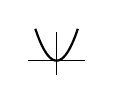
\begin{tikzpicture}[scale=0.18, baseline=-0.3ex]
\draw[thin] (-2,0) -- (2,0); \draw[thin] (0,-1) -- (0,2);
\draw[thick,domain=-1.5:1.5,smooth] plot (\x,{(\x)^2});
\end{tikzpicture}\textbf{Quadratic:} $x^2$\par
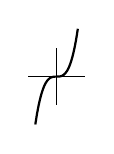
\begin{tikzpicture}[scale=0.18, baseline=-0.3ex]
\draw[thin] (-2,0) -- (2,0); \draw[thin] (0,-2) -- (0,2);
\draw[thick,domain=-1.5:1.5,smooth] plot (\x,{(\x)^3});
\end{tikzpicture}\textbf{Cubic:} $x^3$\par
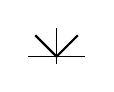
\begin{tikzpicture}[scale=0.18, baseline=-0.3ex]
\draw[thin] (-2,0) -- (2,0); \draw[thin] (0,-0.5) -- (0,2);
\draw[thick] (-1.5,1.5) -- (0,0) -- (1.5,1.5);
\end{tikzpicture}\textbf{Absolute:} $|x|$\par

\begin{tikzpicture}[scale=0.18, baseline=-0.3ex]
\draw[thin] (-0.5,0) -- (2,0); \draw[thin] (0,-0.5) -- (0,2);
\draw[thick,domain=0:1.8,smooth] plot (\x,{sqrt(\x)});
\end{tikzpicture}\textbf{Square root:} $\sqrt{x}$\par
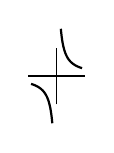
\begin{tikzpicture}[scale=0.18, baseline=-0.3ex]
\draw[thin] (-2,0) -- (2,0); \draw[thin] (0,-2) -- (0,2);
\draw[thick,domain=-1.8:-0.3,smooth] plot (\x,{1/\x});
\draw[thick,domain=0.3:1.8,smooth] plot (\x,{1/\x});
\end{tikzpicture}\textbf{Reciprocal:} $1/x$\par
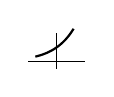
\begin{tikzpicture}[scale=0.18, baseline=-0.3ex]
\draw[thin] (-2,0) -- (2,0); \draw[thin] (0,-0.5) -- (0,2);
\draw[thick,domain=-1.5:1.2,smooth] plot (\x,{exp(\x*0.7)});
\end{tikzpicture}\textbf{Exponential:} $a^x$\par

\begin{tikzpicture}[scale=0.18, baseline=-0.3ex]
\draw[thin] (-0.5,0) -- (2,0); \draw[thin] (0,-2) -- (0,1);
\draw[thick,domain=0.2:1.8,smooth] plot (\x,{ln(\x)});
\end{tikzpicture}\textbf{Logarithmic:} $\ln(x)$\par
}

\boxedsection{Inverse Functions}{%
\textbf{Idea:} $f^{-1}$ reverses $f$ ($x \to y$ becomes $y \to x$)\par
\textbf{Exists when:} $f$ is one-to-one (horizontal line test). If not, restrict domain\par
\textbf{Graph rule:} $f^{-1}$ is $f$ reflected in $y = x$\par
\textbf{Domain/Range:} $f: A \to B$; $f^{-1}: B \to A$\par
}

\boxedsection{Partial Fractions}{%
\textbf{1. Distinct linear:} $\frac{1}{(x-a)(x-b)} = \frac{A}{x-a} + \frac{B}{x-b}$\par
\textbf{2. Repeated linear:} $\frac{1}{(x-a)^n} = \frac{A_1}{x-a} + \frac{A_2}{(x-a)^2} + \cdots + \frac{A_n}{(x-a)^n}$\par
\textbf{3. Irreducible quadratic:} $\frac{1}{x^2+px+q} = \frac{Ax+B}{x^2+px+q}$\par
\textbf{Example:} $\int \frac{3x+5}{x^2-1} dx$\par
Factor: $x^2-1 = (x-1)(x+1)$\par
Decompose: $\frac{3x+5}{(x-1)(x+1)} = \frac{A}{x-1} + \frac{B}{x+1}$\par
Multiply: $3x+5 = A(x+1) + B(x-1)$\par
Expand: $3x+5 = (A+B)x + (A-B)$\par
Match: $A+B=3$, $A-B=5$ $\Rightarrow$ $A=4$, $B=-1$\par
}

\boxedsection{Limits: $x \to \infty$}{%
\textbf{Exponentials:} $a^x$ ($a>1$) $\to \infty$; $e^{-x} \to 0$; beat everything\par
\textbf{Logs:} $\ln x \to \infty$ (very slow); polynomials/exponentials faster\par
\textbf{Roots:} $\sqrt{x} \to \infty$ (slower than $x$); $1/\sqrt{x} \to 0$\par
}

\section{Derivatives}

\boxedsection{Trig Derivatives}{%
$(\sin x)' = \cos x$\par
$(\cos x)' = -\sin x$\par
$(\tan x)' = \sec^2 x$\par
$(\cot x)' = -\csc^2 x$\par
$(\sec x)' = \sec x \tan x$\par
$(\csc x)' = -\csc x \cot x$\par
}

\boxedsection{Inverse Trig Derivatives}{%
$(\sin^{-1} x)' = \frac{1}{\sqrt{1-x^2}}$\par
$(\cos^{-1} x)' = -\frac{1}{\sqrt{1-x^2}}$\par
$(\tan^{-1} x)' = \frac{1}{1+x^2}$\par
$(\cot^{-1} x)' = -\frac{1}{1+x^2}$\par
$(\sec^{-1} x)' = \frac{1}{|x|\sqrt{x^2-1}}$\par
$(\csc^{-1} x)' = -\frac{1}{|x|\sqrt{x^2-1}}$\par
}

\boxedsection{Exponential \& Log Derivatives}{%
$(e^x)' = e^x$\par
$(a^x)' = a^x \ln a$\par
$(\ln x)' = \frac{1}{x}$\par
}

\boxedsection{Logarithmic Differentiation}{%
\textbf{When:} $f(x)$ has variable in base and exponent, or complex products/quotients\par
\textbf{Method:} $f(x) = \sqrt{\frac{1+6\sin^2 x}{(1+\tan x)^2}}$\par
\textbf{Step 1:} $\ln f(x) = \frac{1}{2}\ln(1+6\sin^2 x) - 2\ln(1+\tan x)$\par
\textbf{Step 2:} $\frac{1}{f(x)}f'(x) = \frac{6\sin x\cos x}{1+6\sin^2 x} - \frac{2\sec^2 x}{1+\tan x}$\par
\textbf{Step 3:} $f'(x) = f(x)\left[\frac{6\sin x\cos x}{1+6\sin^2 x} - \frac{2\sec^2 x}{1+\tan x}\right]$\par
}

\boxedsection{Chain Rule Example}{%
\textbf{Differentiate:} $y = \sin(3x^2 + 4x)$\par
\textbf{Outer:} $\sin(u)$, \textbf{Inner:} $u = 3x^2 + 4x$\par
\textbf{Steps:} $y' = \cos(u) \cdot u' = \cos(3x^2 + 4x)(6x + 4)$\par
\textbf{Answer:} $y' = (6x + 4)\cos(3x^2 + 4x)$\par
}

\boxedsection{Implicit Differentiation}{%
\textbf{Used when:} $y$ cannot be isolated easily\par
\textbf{Steps:}\par
1. Differentiate both sides w.r.t. $x$\par
2. Treat $y$ as function of $x$ $\to$ multiply by $\frac{dy}{dx}$ when differentiating $y$\par
3. Collect $\frac{dy}{dx}$ terms\par
4. Solve for $\frac{dy}{dx}$\par
}

\boxedsection{Implicit Diff Example}{%
\textbf{Differentiate:} $x^2 + y^2 = 25$\par
\textbf{Differentiate:} $2x + 2y \cdot \frac{dy}{dx} = 0$\par
\textbf{Solve:} $2y \frac{dy}{dx} = -2x$\par
$\frac{dy}{dx} = -\frac{x}{y}$\par
}

\section{Applications of Derivatives}

\boxedsection{Related Rates Example}{%
\textbf{Question:} Circle expanding. Radius increases at $\frac{dr}{dt} = 2$ cm/s. Find $\frac{dA}{dt}$ when $r = 5$ cm.\par
\textbf{Solution pattern:}\par
1. Formula: $A = \pi r^2$\par
2. Differentiate w.r.t. time $t$: $\frac{dA}{dt} = 2\pi r \frac{dr}{dt}$\par
3. Substitute: $r = 5$, $\frac{dr}{dt} = 2$\par
$\frac{dA}{dt} = 2\pi(5)(2) = 20\pi$ cm$^2$/s\par
\textbf{Answer:} $20\pi$ cm$^2$/s\par
}

\boxedsection{Extrema Procedure}{%
\textbf{Step 1:} Find $f'(x)$ (differentiate)\par
\textbf{Step 2:} Find critical numbers: $f'(x) = 0$ and where $f'(x)$ undefined (in domain)\par
\textbf{Step 3:} Classify (First Derivative Test):\par
$f'$ changes $+ \to -$: local max\par
$f'$ changes $- \to +$: local min\par
No sign change: neither\par
}

\boxedsection{Second Derivative Test}{%
\textbf{If $f''(c)$ exists:}\par
$f''(c) < 0 \to$ local maximum\par
$f''(c) > 0 \to$ local minimum\par
$f''(c) = 0 \to$ inconclusive (use First Derivative Test)\par
}

\boxedsection{Optimization Example}{%
\textbf{Question:} 80 m fencing for rectangular field along river (no fence on river side). Find max area.\par
\textbf{Setup:} $x$ = side $\perp$ river, $y$ = side $\parallel$ river\par
\textbf{Total fence:} $2x + y = 80 \Rightarrow y = 80 - 2x$\par
\textbf{Area:} $A = xy = x(80-2x) = 80x - 2x^2$\par
\textbf{Differentiate:} $A'(x) = 80 - 4x$\par
\textbf{Set to zero:} $80 - 4x = 0 \Rightarrow x = 20$\par
\textbf{Then:} $y = 80 - 2(20) = 40$\par
\textbf{Check:} $A''(x) = -4 < 0$ (max)\par
\textbf{Answer:} $20$ m by $40$ m\par
}

\section{Integral}

\boxedsection{Special Case: $x^{-1}$}{%
$\int \frac{1}{x} dx = \ln |x| + C$\par
\textbf{Warning:} Do NOT apply power rule when $n = -1$\par
}

\boxedsection{Common Integrals (Must Recognize)}{%
$\int e^x dx = e^x + C$\par
$\int a^x dx = \frac{a^x}{\ln a} + C$\par
$\int \sin x dx = -\cos x + C$\par
$\int \cos x dx = \sin x + C$\par
$\int \sec^2 x dx = \tan x + C$\par
}

\boxedsection{Trig Integrals}{%
$\int \cos x dx = \sin x + C$\par
$\int \sin x dx = -\cos x + C$\par
$\int \sec^2 x dx = \tan x + C$\par
$\int \csc^2 x dx = -\cot x + C$\par
$\int \sec x \tan x dx = \sec x + C$\par
$\int \csc x \cot x dx = -\csc x + C$\par
}

\boxedsection{Riemann Sums}{%
\textbf{Interval:} $[a, b]$\par
\textbf{Width:} $\Delta x = \frac{b-a}{n}$\par
\textbf{Sample points:}\par
Left endpoints: $x_i^* = a + (i-1)\Delta x$\par
Right endpoints: $x_i^* = a + i\Delta x$\par
\textbf{Left Riemann Sum:} $L_n = \sum_{i=1}^n f(a + (i-1)\Delta x) \Delta x$\par
\textbf{Right Riemann Sum:} $R_n = \sum_{i=1}^n f(a + i\Delta x) \Delta x$\par
}

\boxedsection{Net Change Theorem}{%
$\int_a^b (\text{rate of change}) dt = \text{total change over } [a, b]$\par
}

\boxedsection{U-Substitution Example 1}{%
\textbf{Integral:} $\int \frac{x}{\sqrt{1+x^2}} dx$\par
\textbf{Let:} $u = 1 + x^2$, $du = 2x dx \Rightarrow x dx = \frac{1}{2} du$\par
\textbf{Rewrite:} $\int \frac{1}{\sqrt{u}} \cdot \frac{1}{2} du = \frac{1}{2} \int u^{-1/2} du$\par
\textbf{Integrate:} $\frac{1}{2} \cdot \frac{u^{1/2}}{1/2} = \sqrt{u} + C$\par
\textbf{Back-substitute:} $\sqrt{1+x^2} + C$\par
}

\boxedsection{U-Substitution Example 2}{%
\textbf{Integral:} $\int \frac{\sin x}{(1+\cos x)^2} dx$\par
\textbf{Let:} $u = 1 + \cos x$, $du = -\sin x dx$\par
\textbf{Then:} $\int \frac{\sin x}{(1+\cos x)^2} dx = -\int \frac{1}{u^2} du$\par
\textbf{Integrate:} $-\frac{u^{-1}}{-1} = u^{-1} + C = \frac{1}{u} + C$\par
\textbf{Back-substitute:} $\frac{1}{1+\cos x} + C$\par
}

\section{Applications of Integrals}

\boxedsection{Disk Method (no hole)}{%
\textbf{Use when:} region touches axis of rotation (solid goes all the way to axis)\par
\textbf{Formula:} $V = \pi \int_a^b [R(x)]^2 dx$\par
\textbf{Meaning:} Each slice forms a solid disk. Radius $R(x)$ is distance from axis to curve.\par
}

\boxedsection{Washer Method (hole present)}{%
\textbf{Use when:} region does not touch axis (empty space in middle)\par
\textbf{Formula:} $V = \pi \int_a^b [R(x)^2 - r(x)^2] dx$\par
\textbf{Meaning:} Each slice is a washer: outer circle minus inner circle.\par
$R(x) =$ outer radius, $r(x) =$ inner radius.\par
}

\boxedsection{Rotation Rules}{%
Rotate about $x$-axis $\to$ radii measured vertically $\to$ use $y = f(x)$\par
Rotate about $y$-axis $\to$ radii measured horizontally $\to$ often rewrite as $x = g(y)$\par
\textbf{Always measure radius perpendicular to axis of rotation.}\par
}

\boxedsection{Average Value}{%
\textbf{Formula:} $f_{\text{avg}} = \frac{1}{b-a} \int_a^b f(x) dx$\par
\textbf{Meaning:}\par
$\bullet$ The "mean height" of graph on $[a, b]$\par
$\bullet$ Constant value whose rectangle has same area as area under $f$\par
}

\section{Differential Equations}

\boxedsection{Simple DE Example}{%
\textbf{Solve:} $\frac{dy}{dx} = 3x^2$\par
\textbf{Integrate both sides:} $y = x^3 + C$\par
}

\boxedsection{Separable DE Example 1}{%
\textbf{Solve:} $\frac{dy}{dx} = y$\par
\textbf{Separate:} $\frac{1}{y} dy = dx$\par
\textbf{Integrate:} $\ln |y| = x + C$\par
\textbf{Exponentiate:} $y = Ce^x$\par
}

\boxedsection{Separable DE Example 2}{%
\textbf{Solve:} $\frac{dy}{dt} = 5 - y$\par
\textbf{Separate:} $\frac{dy}{5-y} = dt$\par
\textbf{Integrate:} $-\ln |5-y| = t + C$\par
\textbf{Rearrange:} $5 - y = Ce^{-t}$\par
\textbf{Final:} $y = 5 - Ce^{-t}$\par
}

\boxedsection{Separable DE Example 3}{%
\textbf{Solve:} $\frac{dy}{dx} = \frac{x}{y+2}$\par
\textbf{Separate:} $(y+2) dy = x dx$\par
\textbf{Integrate:} $\frac{y^2}{2} + 2y = \frac{x^2}{2} + C$\par
\textbf{Multiply by 2:} $y^2 + 4y = x^2 + C$\par
\textbf{Complete square:} $(y+2)^2 = x^2 + K$\par
\textbf{Final:} $y = -2 \pm \sqrt{x^2 + K}$\par
(If initial condition given, solve for $K$.)\par
}

\boxedsection{Logistic Equation Problem}{%
\textbf{Problem:} Fish population modeled by $\frac{dP}{dt} = 0.3P(1 - \frac{P}{500})$ where $P(t)$ is number of fish after $t$ years.\par
\textbf{1. Parameters:} Compare with $P' = rP(1 - P/K)$:\par
$\bullet$ $r = 0.3$ (growth rate)\par
$\bullet$ $K = 500$ (carrying capacity)\par
\textbf{2. Explicit formula:} Given $P(0) = 50$:\par
$P(t) = \frac{P_0 K e^{rt}}{(K-P_0) + P_0 e^{rt}}$\par
Here $P_0 = 50$, $r = 0.3$, $K = 500$:\par
$P(t) = \frac{50 \cdot 500 e^{0.3t}}{(500-50) + 50e^{0.3t}} = \frac{25000e^{0.3t}}{450 + 50e^{0.3t}}$\par
Simplify: $P(t) = \frac{500e^{0.3t}}{9 + e^{0.3t}}$\par
\textbf{3. Population after 5 years:}\par
$P(5) = \frac{500e^{1.5}}{9 + e^{1.5}} \approx \frac{500 \cdot 4.48}{9 + 4.48} = \frac{2240}{13.48} \approx 166$\par
\textbf{4. Long-term behavior:}\par
As $t \to \infty$, $e^{0.3t} \to \infty$. In $P(t) = \frac{500e^{0.3t}}{9 + e^{0.3t}}$, both numerator and denominator dominated by $e^{0.3t}$, so $\lim_{t \to \infty} P(t) = 500$. Population levels off at carrying capacity $K = 500$.\par
}

\boxedsection{First-Order Linear DE}{%
\textbf{Solve:} $\frac{dy}{dx} - 2y = e^{3x}$\par
\textbf{Step 1:} Identify $P(x) = -2$\par
\textbf{Step 2:} Integrating factor: $\mu(x) = e^{\int (-2) dx} = e^{-2x}$\par
\textbf{Step 3:} Multiply DE by $\mu(x)$:\par
$e^{-2x}y' - 2e^{-2x}y = e^{3x}e^{-2x}$\par
Right side simplifies: $e^x$\par
Left side becomes: $\frac{d}{dx}(e^{-2x}y)$\par
}

\section{Series}

\boxedsection{Convergence \& Divergence}{%
\textbf{A series converges if:} $\lim_{n \to \infty} S_n = S$ for some finite number $S$.\par
\textbf{If the partial sums:}\par
$\bullet$ grow without bound $\to$ diverge\par
$\bullet$ oscillate without settling $\to$ diverge\par
\textbf{Necessary Condition for Convergence:}\par
If $\sum a_n$ converges, then $\lim_{n \to \infty} a_n = 0$\par
}

\boxedsection{Geometric Series}{%
\textbf{General form:} $\sum_{n=0}^{\infty} ar^n$\par
\textbf{Convergence rule:}\par
Converges if $|r| < 1$\par
Diverges if $|r| \geq 1$\par
\textbf{Sum when convergent:} $\frac{a}{1-r}$\par
}

\boxedsection{Partial Sums}{%
\textbf{Arithmetic sequence:} $S_n = \frac{n}{2}(2a + (n-1)d)$\par
where $a$ = first term, $d$ = common difference\par
\textbf{Geometric sequence:} $S_n = \frac{a(1-r^n)}{1-r}$\par
where $a$ = first term, $r$ = common ratio\par
}

\boxedsection{Maclaurin Series Example}{%
\textbf{Find first 4 non-zero terms for:} $f(x) = x^2e^{-x}$\par
\textbf{Step 1. Known series:}\par
$e^{-x} = 1 - x + \frac{x^2}{2} - \frac{x^3}{6} + \frac{x^4}{24} - \cdots$\par
\textbf{Step 2. Multiply by $x^2$:}\par
$x^2e^{-x} = x^2\left(1 - x + \frac{x^2}{2} - \frac{x^3}{6} + \frac{x^4}{24} - \cdots\right)$\par
$= x^2 - x^3 + \frac{x^4}{2} - \frac{x^5}{6} + \frac{x^6}{24} - \cdots$\par
\textbf{First 4 non-zero terms:} $x^2 - x^3 + \frac{x^4}{2} - \frac{x^5}{6} + \cdots$\par
}

\section{Vectors}

\boxedsection{Magnitude (length)}{%
$|\vec{v}| = \sqrt{v_x^2 + v_y^2 + v_z^2}$\par
}

\boxedsection{Vector Addition}{%
$\vec{u} + \vec{v} = \begin{bmatrix} u_x + v_x \\ u_y + v_y \\ u_z + v_z \end{bmatrix}$\par
}

\boxedsection{Dot Product}{%
$\vec{u} \cdot \vec{v} = |\vec{u}| |\vec{v}| \cos \theta$\par
}

\boxedsection{Cross Product Magnitude}{%
$|\vec{u} \times \vec{v}| = |\vec{u}| |\vec{v}| \sin \theta$\par
}

\boxedsection{Cross Product Determinant}{%
$\vec{u} \times \vec{v} = \begin{vmatrix} \mathbf{i} & \mathbf{j} & \mathbf{k} \\ u_x & u_y & u_z \\ v_x & v_y & v_z \end{vmatrix}$\par
}

\boxedsection{Intersection of Two Lines}{%
\textbf{Given:} $\vec{r} = \vec{a} + \lambda\vec{d}$ and $\vec{r} = \vec{c} + \mu\vec{e}$\par
\textbf{Set equal:} $\vec{a} + \lambda\vec{d} = \vec{c} + \mu\vec{e}$\par
}

\boxedsection{Distance Between Two Points}{%
$|\overrightarrow{AB}| = \sqrt{(b_x - a_x)^2 + (b_y - a_y)^2 + (b_z - a_z)^2}$\par
}

\end{multicols*}

\end{document}

